
\begin{frame}\frametitle{Cases of non-Turing-universal oritatami systems}

\begin{figure}[tb]
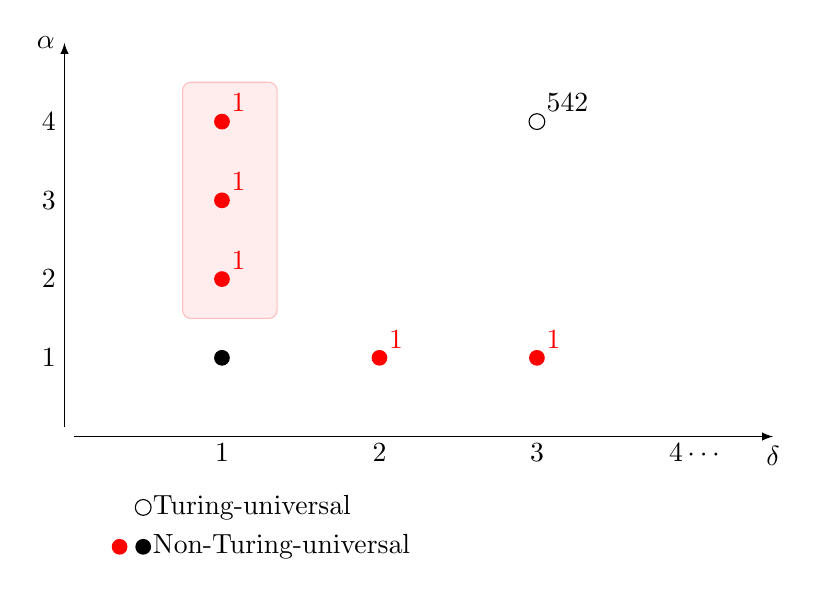
\begin{tikzpicture}
%mark
\fill[pink!30, rounded corners=3pt]
	(1.5, 1.5) -- (1.5, 4.5) -- (2.7, 4.5) -- (2.7, 1.5) -- cycle;
\draw[pink, rounded corners=3pt]
	(1.5, 1.5) -- (1.5, 4.5) -- (2.7, 4.5) -- (2.7, 1.5) -- cycle;


\node (origin) at (0, 0) {};

\draw[-latex] (origin) -- ++(0:9) node[below] {$\delta$}; 
\node at (2, -0.2) {1};
\node at (4, -0.2) {2};
\node at (6, -0.2) {3};
\node at (8, -0.2) {$4 \cdots$};
\draw[-latex] (origin) -- ++(90:5) node[left] {$\alpha$}; 
\node at (-0.2, 1) {1};
\node at (-0.2, 2) {2};
\node at (-0.2, 3) {3};
\node at (-0.2, 4) {4};

\fill (2, 4) [red] circle[radius = 0.1];
\fill (2, 4) [red] node [above right] {1};
\fill (2, 3) [red] circle[radius = 0.1];
\fill (2, 3) [red] node [above right] {1};

\fill (2, 2) [red] circle[radius = 0.1];
\fill (2, 2) [red] node [above right] {1};
\fill (2, 1) circle[radius = 0.1];

\fill (4, 1) [red] circle[radius = 0.1];
\fill (4, 1) [red] node [above right] {1};

\draw (6, 4) circle[radius = 0.1];
\fill (6, 4) node [above right] {542};
\fill (6, 1) [red] circle[radius = 0.1];
\fill (6, 1) [red] node [above right] {1};

\draw (1, -0.9) circle[radius = 0.1];
\fill (1, -0.9) node [right] {Turing-universal};
\fill (0.7, -1.4) [red] circle[radius = 0.1];
\fill (1, -1.4) circle[radius = 0.1];
\fill (1, -1.4) node [right] {Non-Turing-universal};

\end{tikzpicture}
\end{figure}

\end{frame}



%%%%%%%%%%
%%%
%%%%%%%%%%

\section{Proof of not Turing universality}

\subsection{Stabilization methods}

\begin{frame}\frametitle{Oritatami systems at delay 1}
  \begin{block}{The two ways for a bead stabilization at delay 1}
    \begin{itemize}
    \item To be bound to another bead.
    \item Through a 1-in-1-out structure called the tunnel section.
    \end{itemize}
  \end{block}

\begin{center}
	\begin{columns}[c]
		\begin{column}{0.3\textwidth}
	    \begin{tikzpicture}
      	\fill (0,0) circle [radius=0.05];
        \fill[shift=(60:1)] (120:1) circle [radius=0.1];
         \fill[blue] (60:1) circle [radius=0.05];
        \fill (120:1) circle [radius=0.1];
      
      \draw[->,] (180:0.9) -- (180:0.1);
      \draw[->, blue] (60:0.1) -- (60:0.9);
       \draw[dotted, thick, shift = (60:1)] (0:0) -- (120:1);
%    	\node[right] at (60:1) {$w[i]$};
	
	\node at (0,-1) {Bond};
%	\node at (0,-1.5) {$S[i] = b$};
	
	\draw[white] (180:1) -- (180:2);
	\end{tikzpicture}
	
	\end{column}
	
	\begin{column}{0.3\textwidth}
	\begin{tikzpicture}
          \begin{scope}[yshift=2cm]
          
            \draw[white] (60:1) -- (0:0);
            \draw[white] (-60:1) -- (0:0);
%            \node[above] at (0,0) {$w[i-1]$};
%            \node[above] at (0:1) {$w[i]$};

          
            
            \foreach \theta in {60,-60,120,-120}{
              \fill[transform canvas={shift=(\theta:1)}](0,0) circle [radius=0.1];
            }
            \only<1>{
            		\draw(0,0) circle [radius=0.05];
			\draw(0:1) circle [radius=0.05];
			\draw(0:-1) circle [radius=0.05];
            }
            \only<2>{
	            \fill(0,0) circle [radius=0.05];
                 \fill[transform canvas={shift=(180:1)}, red](0,0) circle [radius=0.1];
         	      \fill[blue, transform canvas={shift=(0:1)}](0,0) circle [radius=0.05];
	     		\draw[dotted, thick] (60:0.1) -- (60:0.9);
	          \draw[->] (-0.9, 0) -- (-0.1, 0);
	          \draw[->, blue] (0.1, 0) -- (0.9, 0);
          }
          \end{scope}
          

          \node at (0,0) {Tunnel section};
        \end{tikzpicture}
	\end{column}
	
%	\begin{column}{0.3\textwidth}
%	\visible<2>{
%		\begin{tikzpicture}
%		\node[anchor=center, inner sep=0)] at (0:0) {
% 		   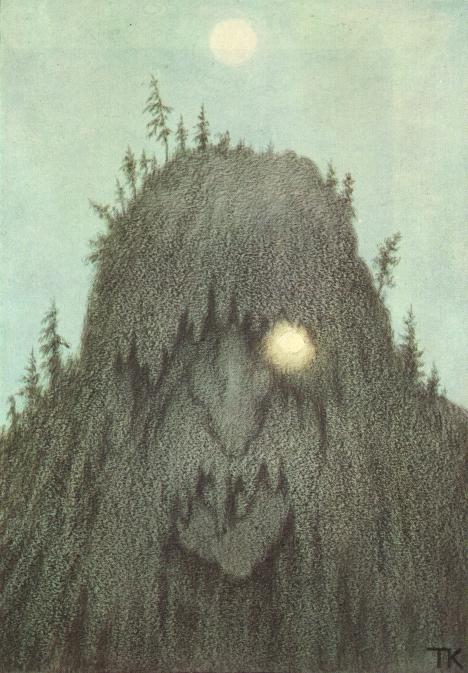
\includegraphics[width=0.6\textwidth]{fig/Forest_Troll.jpg}
%		 };
%		 \node at (-90:2) {Tunnel Troll Theorem};
%	        \end{tikzpicture}
%	 }
%	\end{column}
	\end{columns}
\end{center}

\end{frame}



\begin{frame}\frametitle{Deterministic unary oritatami systems at delay 1}
\begin{block}{Results ($\delta = 1$)}
\begin{table}[h]
\begin{tabular}{l l}
$\alpha = 4$ & $3n^2{+}3n{+}1$ \\
$\alpha = 3$ & $4n{+}14$ \\
$\alpha = 2$ & $\infty$ but zigzag after $(27n^2{+}9n{+}1)$ \\
 *\footnote{c.f. $\alpha = 1$: $10n$ (Demaine et al. 2018 DNA24)}\\ %*\footnote{\cite{DHOPRSST2018}} \\
\end{tabular}
\end{table}
\end{block}

\begin{center}
    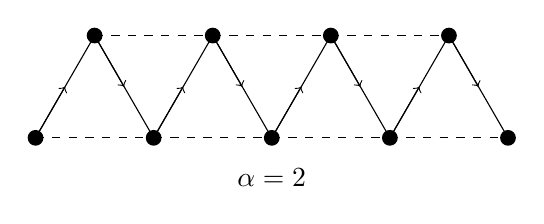
\begin{tikzpicture}
      \fill (0,0) circle[radius = 0.1];
      \fill (1.5,0) circle[radius = 0.1];
      \fill (3,0) circle[radius = 0.1];
      \fill (4.5,0) circle[radius = 0.1];
      \fill (6,0) circle[radius = 0.1];

      \draw[dashed] (0,0)--(1.5,0);
      \draw[dashed] (1.5,0)--(3,0);
      \draw[dashed] (3,0)--(4.5,0);
      \draw[dashed] (4.5,0)--(6,0);
      \draw[->] (0,0)--(60:0.75);
      \draw[->] (1.5,0)--++(60:0.75);
      \draw[->] (3,0)--++(60:0.75);
      \draw[->] (4.5,0)--++(60:0.75);
      \draw (0,0)--(60:1.5);
      \draw (1.5,0)--++(60:1.5);
      \draw (3,0)--++(60:1.5);
      \draw (4.5,0)--++(60:1.5);
      
      \begin{scope}[shift=(60:1.5)]
        \fill (0,0) circle[radius = 0.1];
        \fill (1.5,0) circle[radius = 0.1];
        \fill (3,0) circle[radius = 0.1];
        \fill (4.5,0) circle[radius = 0.1];
        \draw[dashed] (0,0)--(1.5,0);
        \draw[dashed] (1.5,0)--(3,0);
        \draw[dashed] (3,0)--(4.5,0);
        \draw[->] (0,0)--(-60:0.75);
        \draw[->] (1.5,0)--++(-60:0.75);
        \draw[->] (3,0)--++(-60:0.75);
        \draw[->] (4.5,0)--++(-60:0.75);
        
        \draw (0,0)--(-60:1.5);
        \draw (1.5,0)--++(-60:1.5);
        \draw (3,0)--++(-60:1.5);
        \draw (4.5,0)--++(-60:1.5);
      \end{scope}
      
      \node at (3,-0.5) {$\alpha = 2$};
    \end{tikzpicture}
\end{center}

\end{frame}

\subsection{$\alpha = 2$}

%%%%%%%%%% zig-zag a = 2

\begin{frame}\frametitle{zig-zag}
\begin{block}{}
Deterministic \alert{unary} oritatami system at $\delta = 1$ and at $\alpha = 2$ can make zig-zag but cannot at larger arity

\end{block}

\centering{
    \begin{tikzpicture}
    \begin{scope}[blue, dashed]
    	\draw (0:0) -- (0:2);
	\draw (0:2) -- (0:4);
	
    	\draw[shift=(60:2)] (0:0) -- (0:2);
	\visible<3->{
		\draw[shift=(60:2)] (0:2) -- (0:4);
	}
	\visible<4>{
		\draw (0:4) -- (0:6);
	}
    \end{scope}
    \begin{scope}[red]
    	\draw (0:0) -- (60:2);
	\draw[shift=(0:2)] (0:0) -- (120:2);
	\draw[shift=(0:2)] (0:0) -- (60:2);
	\draw[shift=(0:4)] (0:0) -- (120:2);
    
    	\fill (0:0) circle [radius=0.1];
	\fill (0:2) circle [radius=0.1];
	\fill (0:4) circle [radius=0.1];
	\fill[shift=(60:2)] (0:0) circle [radius=0.1];
	\fill[shift=(60:2)] (0:2) circle [radius=0.1];
    \end{scope}
      
      \begin{scope}[blue]
      \node[below] at (0:0) {+1};
      \node[above, shift=(60:2)] at (0:0) {+1};
      \node[below] at (0:2) {+0};
      \only<-2>{
  	    \node[above, shift=(60:2)] at (0:2) {+1};
      }
      \only<3->{
	    \node[above, shift=(60:2)] at (0:2) {+0};
      }
      \only<-3>{
 	     \node[below] at (0:4) {+1};
      }
      \only<4>{
  	     \node[below] at (0:4) {+0};
      }
      \only<2>{
      		\node[above, shift=(60:2)] at (0:4) {+2};
      }
      \only<3->{
      		\node[above, shift=(60:2)] at (0:4) {+1};
      }
      \visible<4>{
  	     \node[below] at (0:6) {+1};
      }
      \end{scope}
      
      \visible<2->{
      		\fill[shift=(0:4)] (60:2) circle [radius=0.1];
		\draw[->, shift=(0:4)] (60:0.2) -- (60:1.8);
      }
      \visible<4>{
      		\fill[shift=(0:4)] (0:2) circle [radius=0.1];
		\draw[->, shift=(0:6)] (120:1.8) -- (120:0.2);
      }
          
      \node at (3,-1.5) {$\alpha = 2$};
    \end{tikzpicture}
}
\end{frame}

%%% zig-zag a = 3

\begin{frame}\frametitle{zig-zag}
\begin{block}{}
Deterministic \alert{unary} oritatami system at $\delta = 1$ and at $\alpha = 2$ can make zig-zag but cannot at larger arity
\end{block}
\centering{
    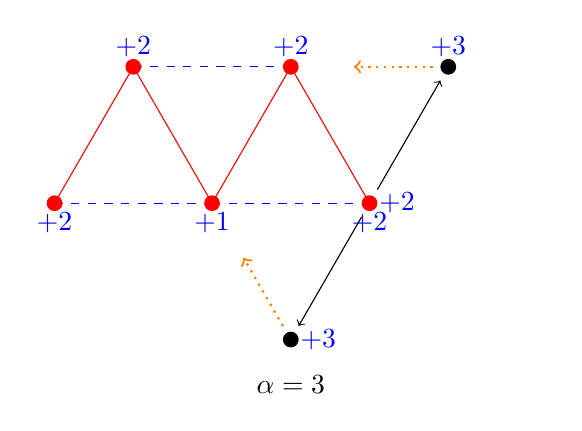
\begin{tikzpicture}
    %adj
    \draw[white] (0:6) circle [radius=0.1];
    \node[below, white] at (0:6) {+1};
    
    \begin{scope}[blue, dashed]
    	\draw (0:0) -- (0:2);
	\draw (0:2) -- (0:4);
	
    	\draw[shift=(60:2)] (0:0) -- (0:2);
    \end{scope}
    \begin{scope}[red]
    	\draw (0:0) -- (60:2);
	\draw[shift=(0:2)] (0:0) -- (120:2);
	\draw[shift=(0:2)] (0:0) -- (60:2);
	\draw[shift=(0:4)] (0:0) -- (120:2);
    
    	\fill (0:0) circle [radius=0.1];
	\fill (0:2) circle [radius=0.1];
	\fill (0:4) circle [radius=0.1];
	\fill[shift=(60:2)] (0:0) circle [radius=0.1];
	\fill[shift=(60:2)] (0:2) circle [radius=0.1];
    \end{scope}
      
      \begin{scope}[blue]
      \node[below] at (0:0) {+2};
      \node[above, shift=(60:2)] at (0:0) {+2};
      \node[below] at (0:2) {+1};
  	\node[above, shift=(60:2)] at (0:2) {+2};
      
      \end{scope}
      
      	\visible<1>{
	      	\fill[shift=(0:4)] (60:2) circle [radius=0.1];
		\draw[->, shift=(0:4)] (60:0.2) -- (60:1.8);
		\node[above, shift=(60:2), blue] at (0:4) {+3};
		\node[below, blue] at (0:4) {+2};
		\draw[->, thick, dotted, orange, shift=(60:2)] (0:3.8) -- (0:2.8);
	}
	\visible<2>{
      		\fill[shift=(0:4)] (-120:2) circle [radius=0.1];
		\draw[->, shift=(0:4)] (-120:0.2) -- (-120:1.8);
		\node[right, shift=(-120:2), blue] at (0:4) {+3};
		\node[right, blue] at (0:4) {+2};
		\draw[->, thick, dotted, orange, shift=(0:2)] (-60:1.8) -- (-60:0.8);
	}
          
      \node at (3,-2.3) {$\alpha = 3$};
    \end{tikzpicture}
}
\end{frame}


%%%%%%%%%%


%\begin{frame}\frametitle{Deterministic unary oritatami systems at delay 1}
%\centering
%\begin{tikzpicture}
%    \begin{scope}[blue, dashed]
%    	\draw (0:0) -- (0:2);
%	\draw (0:2) -- (0:4);
%	
%    	\draw[shift=(60:2)] (0:0) -- (0:2);
%    \end{scope}
%    \begin{scope}[]
%    	\draw (0:0) -- (60:2);
%	\draw[shift=(0:2)] (0:0) -- (120:2);
%	\draw[shift=(0:2)] (0:0) -- (60:2);
%	\draw[shift=(0:4)] (0:0) -- (120:2);
%    
%    	\fill (0:0) circle [radius=0.1];
%	\fill (0:2) circle [radius=0.1];
%	\fill (0:4) circle [radius=0.1];
%	\fill[shift=(60:2)] (0:0) circle [radius=0.1];
%	\fill[shift=(60:2)] (0:2) circle [radius=0.1];
%    \end{scope}
%      
%      		\fill[shift=(0:4)] (60:2) circle [radius=0.1];
%		\draw[->, shift=(0:4)] (60:0.2) -- (60:1.8);
%      
%          
%    \end{tikzpicture}
%
%
%\begin{block}{}
%If there are ($\alpha + 2$) beads in neighbors of a bead, then this bead has no hand.
%\end{block}
%  
%\begin{columns}[c]
%
%	\begin{column}{0.3\textwidth}
%	\begin{tikzpicture}
%		\foreach \tta in {120,180,-120,-60} {
%			\fill(\tta:1) circle [radius=0.05];
%		}
%		\foreach \tta in {120,180} {
%		 \draw[dotted, thick] (\tta:0.9) -- (\tta:0.2);
%		}
%		\fill[red] (0:0) circle [radius=0.1];
%		\draw[olive] (0:1) circle [radius=0.1];
%		\draw[olive] (60:1) circle [radius=0.1];
%		\draw[->] (-120:0.9) -- (-120:0.2);
%		\draw[->] (-60:0.2) -- (-60:0.9);
%		
%		\node at (-90:2) {$\alpha = 2$};
%	\end{tikzpicture}
%	\end{column}
%	
%	\begin{column}{0.3\textwidth}
%	\begin{tikzpicture}
%		\foreach \tta in {60,120,180,-120,-60} {
%			\fill(\tta:1) circle [radius=0.05];
%		}
%		\foreach \tta in {60,120,180} {
%		 \draw[dotted, thick] (\tta:0.9) -- (\tta:0.2);
%		}
%		\fill[red] (0:0) circle [radius=0.1];
%		\draw[olive] (0:1) circle [radius=0.1];
%		\draw[->] (-120:0.9) -- (-120:0.2);
%		\draw[->] (-60:0.2) -- (-60:0.9);
%		
%		\node at (-90:2) {$\alpha = 3$};
%	\end{tikzpicture}
%	\end{column}
%	
%	\begin{column}{0.3\textwidth}
%	\begin{tikzpicture}
%		\foreach \tta in {0,60,120,180,-120,-60} {
%			\fill(\tta:1) circle [radius=0.05];
%		}
%		\foreach \tta in {0,60,120,180} {
%		 \draw[dotted, thick] (\tta:0.9) -- (\tta:0.2);
%		}
%		\fill[red] (0:0) circle [radius=0.1];
%		\draw[->] (-120:0.9) -- (-120:0.2);
%		\draw[->] (-60:0.2) -- (-60:0.9);
%		
%		\node at (-90:2) {$\alpha = 4$};
%	\end{tikzpicture}
%	\end{column}
%\end{columns}
%
%
%\end{frame}


\begin{frame}\frametitle{Deterministic unary oritatami systems at delay 1}
\begin{block}{Results ($\delta = 1$)}
\begin{table}[h]
\begin{tabular}{l l}
\alert{$\alpha = 4$} & \alert{$3n^2{+}3n{+}1$}\\
$\alpha = 3$ & $4n{+}14$ \\
$\alpha = 2$ & $\infty$ but zigzag after $(27n^2{+}9n{+}1)$ \\
 *\footnote{c.f. $\alpha = 1$: $10n$ (Demaine et al. 2018 DNA24)}\\ %*\footnote{\cite{DHOPRSST2018}} \\
\end{tabular}
\end{table}
\end{block}

\begin{center}
    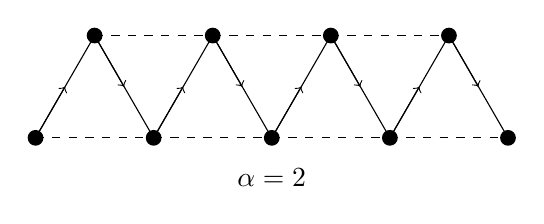
\begin{tikzpicture}
      \fill (0,0) circle[radius = 0.1];
      \fill (1.5,0) circle[radius = 0.1];
      \fill (3,0) circle[radius = 0.1];
      \fill (4.5,0) circle[radius = 0.1];
      \fill (6,0) circle[radius = 0.1];

      \draw[dashed] (0,0)--(1.5,0);
      \draw[dashed] (1.5,0)--(3,0);
      \draw[dashed] (3,0)--(4.5,0);
      \draw[dashed] (4.5,0)--(6,0);
      \draw[->] (0,0)--(60:0.75);
      \draw[->] (1.5,0)--++(60:0.75);
      \draw[->] (3,0)--++(60:0.75);
      \draw[->] (4.5,0)--++(60:0.75);
      \draw (0,0)--(60:1.5);
      \draw (1.5,0)--++(60:1.5);
      \draw (3,0)--++(60:1.5);
      \draw (4.5,0)--++(60:1.5);
      
      \begin{scope}[shift=(60:1.5)]
        \fill (0,0) circle[radius = 0.1];
        \fill (1.5,0) circle[radius = 0.1];
        \fill (3,0) circle[radius = 0.1];
        \fill (4.5,0) circle[radius = 0.1];
        \draw[dashed] (0,0)--(1.5,0);
        \draw[dashed] (1.5,0)--(3,0);
        \draw[dashed] (3,0)--(4.5,0);
        \draw[->] (0,0)--(-60:0.75);
        \draw[->] (1.5,0)--++(-60:0.75);
        \draw[->] (3,0)--++(-60:0.75);
        \draw[->] (4.5,0)--++(-60:0.75);
        
        \draw (0,0)--(-60:1.5);
        \draw (1.5,0)--++(-60:1.5);
        \draw (3,0)--++(-60:1.5);
        \draw (4.5,0)--++(-60:1.5);
      \end{scope}
      
      \node at (3,-0.5) {$\alpha = 2$};
    \end{tikzpicture}
\end{center}

\end{frame}



%%%%%%%%%%%%%%%%%%%%%%%%%%%%%%%%%%%%%%
%%%%%%%%%%%%%%%%%%%%%%%%%



\subsection{$\delta = 1$ and $\alpha = 4$}

%%%hexagon

\begin{frame}\frametitle{Deterministic unary oritatami systems at delay 1}
\begin{block}{$\alpha = 4$}
The terminal conformation at $\alpha = 4$ is of length at most $3n^2  + 3n + 1$($\hexagon_{O}^n$).
\end{block}	

\begin{center}
\begin{tikzpicture}
	%adj
	\begin{scope}[shift=(0:6), white]
	\draw (0:0) -- (-60:1) -- (0:1);
	\draw[dotted, thick] (-60:1) -- (-120:1);
	\draw[dotted, thick] (0:1) -- (0:0);	
	\fill (0:1) circle [radius=0.1];
	\fill (-60:1) circle [radius=0.1];
	\end{scope}
	
	\draw[white, shift=(0:7)] (0:0) -- (-60:0.3);
	\draw[dashed, white, shift=(0:7)] (-60:0.8) -- (-60:0.3);
	%--adj


	\foreach \th in {0,60,120,180,240,300}{
		\draw[dashed] (0:0) -- (\th:3);
		\draw (\th:3) -- (\th + 60:3);
	}
	
	\draw[violet, ->, shift=(150:0.1)] (-120:1.2) -- (-120:0.1);
	\draw[violet, ->, shift=(150:0.1)] (-120:1.8) -- (-120:2.9);
	\node[violet, shift=(150:0.2)] at (-120:1.5) {$n$};
	
	\draw[red] (0:0)
		to[out=-15, in=90] (-20:1)
		to[out=-90, in=90] (-75:0.8)
		to[out=-90, in=160] (-50:1.6);
	\node[red] at (-60:1.8) {seed (n beads)};
	
	\node at (20:4.3) {bead free};
	
	\fill[orange] (0:0) circle [radius=0.1];
	\node[orange, above] at (0:0) {first bead};
	
	\visible<2->{
	\draw[blue] (-50:1.6)
			to[out=-20, in=-120] (-40:2.0)
			to[out=60, in=180] (-30:1.73);
	\draw[blue, shift=(0:2)]
			 (-120:1) -- (-60:1) -- (0:0)
			to[out=40 in=150] (0:1);
	\fill[blue, shift=(0:3)] (-120:1) circle [radius=0.1];
	\fill[blue, shift=(0:2)] (0:0) circle [radius=0.1];
	}
	\visible<2>{
	\draw[blue, shift=(0:3)] (0:0) -- (-60:1);
	\fill[blue, shift=(0:3)] (-60:1) circle [radius=0.1];
	\node[anchor=west, inner sep=0, shift=(0:2), shift=(-60:1), rotate=-90] at (0:0.5) {
 		   
\includegraphics[width=0.04\textwidth]{fig/akusyu1.png}
	};
	\node[anchor=south, inner sep=0, shift=(0:2), rotate=30] at (120:0.2) {
 		   
\includegraphics[width=0.04\textwidth]{fig/te.png}
	};
	}
	\visible<3>{
		\draw[blue, shift=(0:3)] (0:0) -- (120:1);
		\fill[blue, shift=(0:3)] (120:1) circle [radius=0.1];
	\node[anchor=south, inner sep=0, shift=(0:2), shift=(-60:1), rotate=-120] at (-30:0.2) {
 		   
\includegraphics[width=0.04\textwidth]{fig/te.png}
	};
	\node[anchor=west, inner sep=0, shift=(0:2), rotate=-30] at (60:0.5) {
 		   
\includegraphics[width=0.04\textwidth]{fig/akusyu1.png}
	};
	}
	
\end{tikzpicture}
\end{center}

\end{frame}


%%% a = 4

%\begin{frame}\frametitle{Deterministic unary oritatami systems at delay 1}
%\begin{block}{$\alpha = 4$ $(\delta = 1)$}
%The terminal conformation at $\alpha = 4$ is of length at most $3n^2  + 3n + 1$($\hexagon_{O}^n$).
%\end{block}
%
%\begin{center}
%    \begin{tikzpicture}
%
%	\fill (0,0) circle [radius=0.1];
%        \fill[blue] (60:1) circle [radius=0.05];
%        \fill (0:1) circle [radius=0.1];
%        
%	\draw[dotted, thick] (1, 0) -- ++(120:1);
%      
%      \draw[dashed] (180:2) -- (0:2);
%      \draw[dashed, shift=(60:1)] (180:2.5) -- (0:1.5);
%      \draw[->, blue] (60:0.1) -- (60:0.9);
%
%	\node[above] at (180:1) {$p_1$};
%	\node[left] at (-120:1) {$p_2$};
%	\node[left, shift=(-120:1)] at (-60:1) {$p_3$};
%	\node[right] at (-60:1) {$p_4$};
%
%	\draw (180:1) circle [radius=0.05];
%	\draw (-120:1) circle [radius=0.05];
%	\draw (-60:1) circle [radius=0.05];
%	\draw[shift=(-120:1)] (-60:1) circle [radius=0.05];
%
%	\node at (0:2.5) {$n$};
%	\node[shift=(60:1)] at (0:2) {$n+1$};
%    \end{tikzpicture}
%    \end{center}
%\end{frame}



%%%%%%%%%%%%%%%%%% a = 2


\begin{frame}\frametitle{Deterministic unary oritatami systems at delay 1}
\begin{block}{$\alpha = 2$ $(\delta = 1)$}
A transcript folds into the zig-zag conformation after its $(27n^2 + 9n +1)$-th bead ($\hexagon_{O}^{3n}$).
\end{block}

\begin{center}
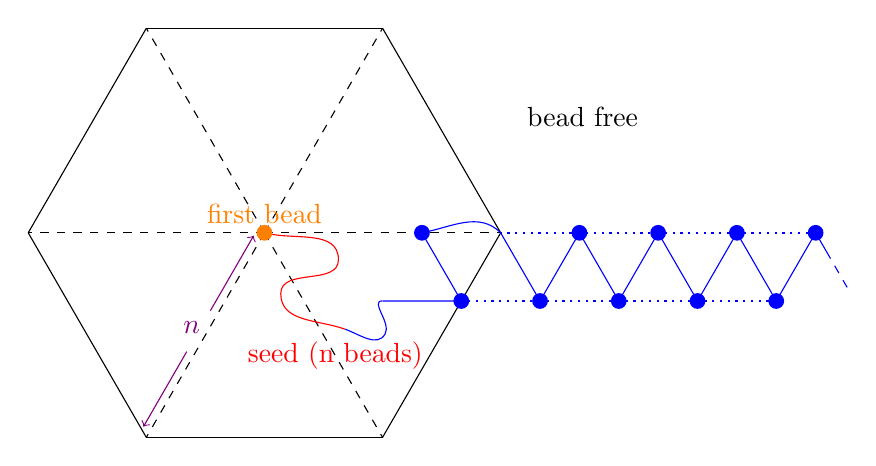
\begin{tikzpicture}
	\foreach \th in {0,60,120,180,240,300}{
		\draw[dashed] (0:0) -- (\th:3);
		\draw (\th:3) -- (\th + 60:3);
	}
	
	\draw[violet, ->, shift=(150:0.1)] (-120:1.2) -- (-120:0.1);
	\draw[violet, ->, shift=(150:0.1)] (-120:1.8) -- (-120:2.9);
	\node[violet, shift=(150:0.2)] at (-120:1.5) {$n$};
	
	\draw[red] (0:0)
		to[out=-15, in=90] (-20:1)
		to[out=-90, in=90] (-75:0.8)
		to[out=-90, in=160] (-50:1.6);
	\node[red] at (-60:1.8) {seed (n beads)};
	
	\node at (20:4.3) {bead free};
	
	\fill[orange] (0:0) circle [radius=0.1];
	\node[orange, above] at (0:0) {first bead};
	
	\draw[blue] (-50:1.6)
			to[out=-20, in=-120] (-40:2.0)
			to[out=60, in=180] (-30:1.73);
	\draw[blue, shift=(0:2)]
			 (-120:1) -- (-60:1) -- (0:0)
			to[out=40 in=150] (0:1);
	\fill[blue, shift=(0:3)] (-120:1) circle [radius=0.1];
	\fill[blue, shift=(0:2)] (0:0) circle [radius=0.1];
			
	\begin{scope}[shift=(0:3), blue]
	\draw (0:0) -- (-60:1) -- (0:1);
	\draw[dotted, thick] (-60:1) -- (-120:1);
	\draw[dotted, thick] (0:1) -- (0:0);	
	\fill (0:1) circle [radius=0.1];
	\fill (-60:1) circle [radius=0.1];
	\end{scope}
	
	\begin{scope}[shift=(0:4), blue]
	\draw (0:0) -- (-60:1) -- (0:1);
	\draw[dotted, thick] (-60:1) -- (-120:1);
	\draw[dotted, thick] (0:1) -- (0:0);	
	\fill (0:1) circle [radius=0.1];
	\fill (-60:1) circle [radius=0.1];
	\end{scope}
	
	\begin{scope}[shift=(0:5), blue]
	\draw (0:0) -- (-60:1) -- (0:1);
	\draw[dotted, thick] (-60:1) -- (-120:1);
	\draw[dotted, thick] (0:1) -- (0:0);	
	\fill (0:1) circle [radius=0.1];
	\fill (-60:1) circle [radius=0.1];
	\end{scope}
	
	\begin{scope}[shift=(0:6), blue]
	\draw (0:0) -- (-60:1) -- (0:1);
	\draw[dotted, thick] (-60:1) -- (-120:1);
	\draw[dotted, thick] (0:1) -- (0:0);	
	\fill (0:1) circle [radius=0.1];
	\fill (-60:1) circle [radius=0.1];
	\end{scope}
	
	\draw[blue, shift=(0:7)] (0:0) -- (-60:0.3);
	\draw[dashed, blue, shift=(0:7)] (-60:0.8) -- (-60:0.3);
	
\end{tikzpicture}
\end{center}

\end{frame}

\begin{frame}\frametitle{Deterministic unary oritatami systems at delay 1}
\begin{block}{$\alpha = 2$ $(\delta = 1)$}
A transcript folds into the zig-zag conformation after its $(27n^2 + 9n +1)$-th bead ($\hexagon_{O}^{3n}$).
\end{block}

\centering
\begin{columns}[c]
    \begin{column}{0.48\textwidth}
    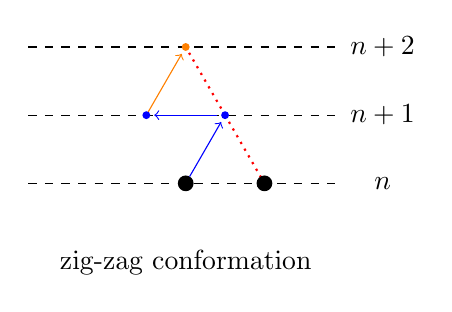
\begin{tikzpicture}
    	\draw[dashed] (180:2) -- (0:2);
      \draw[dashed, shift=(60:1)] (180:2.5) -- (0:1.5);
       \draw[dashed, shift=(60:2)] (180:3) -- (0:1);
    
    	\draw[dotted, red, thick, shift = (60:1)] (0:0) -- (-60:1);
	
%	\visible<2>{
		\draw[red, dotted, thick, shift=(60:1)] (0:0) -- (120:1);
		\draw[->, orange, shift=(60:1), shift=(0:-1)] (0:0) -- (60:0.9);
		
		\fill[orange, shift=(60:1)] (120:1) circle [radius=0.05];
%	}
%	\visible<3>{
%		\draw[red, dotted, thick, shift=(0:-1)] (0:0) -- (-60:1);
%		\draw[red, dotted, thick, shift=(0:-1)] (0:0) -- (-120:1);
%		\draw[->, orange, shift=(120:1)] (0:0) -- (-120:0.9);
%		
%		\fill[orange] (0:-1) circle [radius=0.05];
%	}
    
      	\fill (0,0) circle [radius=0.1];
        \fill[blue] (60:1) circle [radius=0.05];
         \fill[blue] (120:1) circle [radius=0.05];
        \fill (0:1) circle [radius=0.1];
      

      \draw[->, blue] (60:0.1) -- (60:0.9);
      \draw[->, blue, shift=(60:1)] (180:0.1) -- (180:0.9);      

	%\node[above,shift=(120:1)]at (60:1) {$p$};

	%\draw[shift=(120:1)] (60:1) circle [radius=0.05];

	\node at (0:2.5) {$n$};
	\node[shift=(60:1)] at (0:2) {$n+1$};
	\node[shift=(60:2)] at (0:1.5) {$n+2$};
	
	%\node[below] at (0:0) {$w[i-1]$};
	%\node[above] at (60:1) {$w[i]$};
	%\node[above] at (120:1) {$w[i+1]$};
	
	\node at (-90:1) {zig-zag conformation};
	\end{tikzpicture}
    \end{column}
    
    \begin{column}{0.48\textwidth}
    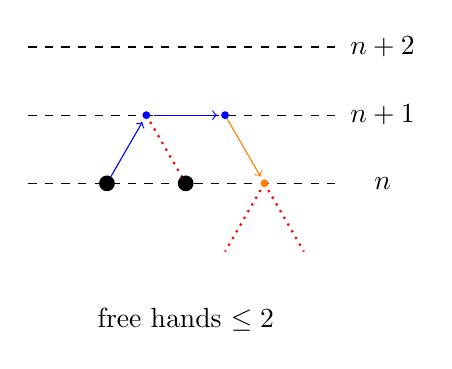
\begin{tikzpicture}
    	 \draw[dashed] (180:1) -- (0:3);
      \draw[dashed, shift=(60:1)] (180:1.5) -- (0:2.5);
       \draw[dashed, shift=(60:2)] (180:2) -- (0:2);
    
    	\draw[dotted, red, thick, shift = (60:1)] (0:0) -- (-60:1);
	
%	\visible<2>{
%		\draw[red, dotted, thick, shift=(60:1)] (0:0) -- (60:1);
%		\draw[->, orange, shift=(60:1), shift=(0:1)] (120:0) -- (120:0.9);
%		
%		\fill[orange] (60:2) circle [radius=0.05];
%	}
%	\visible<3>{
		\draw[red, dotted, thick, shift=(0:2)] (0:0) -- (-60:1);
		\draw[red, dotted, thick, shift=(0:2)] (0:0) -- (-120:1);
		\draw[->, orange, shift=(60:1), shift=(0:1)] (0:0) -- (-60:0.9);
		
		\fill[orange] (0:2) circle [radius=0.05];
%	}
    
      	\fill (0,0) circle [radius=0.1];
        \fill[blue] (60:1) circle [radius=0.05];
         \fill[blue, shift=(0:1)] (60:1) circle [radius=0.05];
        \fill (0:1) circle [radius=0.1];
      
     
      \draw[->, blue] (60:0.1) -- (60:0.9);
      \draw[->, blue, shift=(60:1)] (0:0.1) -- (0:0.9);
      

	%\node[above] at (60:2) {$p$};

	%\draw (60:2) circle [radius=0.05];

	\node at (0:3.5) {$n$};
	\node[shift=(60:1)] at (0:3) {$n+1$};
	\node[shift=(60:2)] at (0:2.5) {$n+2$};
	
	%\node[below] at (0:0) {$w[i-1]$};
	%\node[above] at (60:1) {$w[i]$};
	%\node[above, shift=(0:1)] at (60:1) {$w[i+1]$};
	
	\node at (-60:2) {free hands $\leq 2$};
	\end{tikzpicture}
	\end{column}
	\end{columns}
	
%\visible<2>{
%	zig-zag conformation
%}


\end{frame}

%%%%%%%


\begin{frame}\frametitle{Deterministic unary oritatami systems at delay 1}
\begin{block}{$\alpha = 2$ $(\delta = 1)$}
A transcript folds into the zig-zag conformation after its $(27n^2 + 9n +1)$-th bead ($\hexagon_{O}^{3n}$).
\end{block}

	\begin{columns}[c]
	\begin{column}{0.28\textwidth}
	\begin{tikzpicture}
		\node[anchor=south, inner sep=0, rotate=45] at (135:0.2) {
 		   
\includegraphics[width=0.17\textwidth]{fig/te.png}
		 };
		 
		 \node[anchor=west, inner sep=0, rotate=-30] at (60:0.5) {
 		   
\includegraphics[width=0.15\textwidth]{fig/akusyu1.png}
		 };
	
%		\draw[thick, dotted] (0:0) -- (60:1);
		\draw (0:0) -- (-120:1);
		
		\fill[blue] (0:0) circle [radius=0.1];
		\fill (60:1) circle [radius=0.1];
		
		\node at (-90:2) {free hands = $\pm0$};
	\end{tikzpicture}
	\end{column}
	
	\begin{column}{0.28\textwidth}
	\begin{tikzpicture}
		 \node[anchor=east, inner sep=0, rotate=30] at (120:0.5) {
 		   
\includegraphics[width=0.15\textwidth]{fig/akusyur.png}
		 };
		 \node[anchor=west, inner sep=0, rotate=-30] at (60:0.5) {
 		   
\includegraphics[width=0.15\textwidth]{fig/akusyu1.png}
		 };
	
%		\draw[thick, dotted] (0:0) -- (60:1);
%		\draw[thick, dotted] (0:0) -- (120:1);
		\draw (0:0) -- (-120:1);
		
		\fill[blue] (0:0) circle [radius=0.1];
		\fill (60:1) circle [radius=0.1];
		\fill (120:1) circle [radius=0.1];
		\node at (-90:2) {free hands = $-2$};
	\end{tikzpicture}
	\end{column}
	
	\begin{column}{0.4\textwidth}
	\begin{tikzpicture}
		\node[anchor=south, inner sep=0, rotate=-30] at (60:0.2) {
 		   
\includegraphics[width=0.12\textwidth]{fig/te.png}
		 };
		 \visible<1>{
			\node[anchor=south, inner sep=0, rotate=-120] at (-60:0.2) {
 			   
\includegraphics[width=0.12\textwidth]{fig/ter.png}
			 };
		 }
		 \visible<2>{
			\node[anchor=south, inner sep=0, rotate=-120] at (-60:0.2) {
 			   
\includegraphics[width=0.12\textwidth]{fig/akusyu1.png}
			 };
			 \node[anchor=center, inner sep=0)] at (-22:1.5) {
 			   
\includegraphics[width=0.2\textwidth]{fig/TrollFace.jpg}
			 };
			 \node[below, shift=(-90:0.3)] at (-22:1.5) {Troll};
		 }
	
		\draw (0:0) -- (180:1);
		\draw (180:2) -- (180:1);
		
		\fill[blue] (0:0) circle [radius=0.1];
		\fill[red] (-120:1) circle [radius=0.1];
		\fill[red] (120:1) circle [radius=0.1];
		\fill[red, shift=(180:1)] (-120:1) circle [radius=0.1];
		\fill[red, shift=(180:1)] (120:1) circle [radius=0.1];
		\fill[shift=(180:1)] (180:1) circle [radius=0.1];
		\fill[shift=(180:1)] (0:0) circle [radius=0.1];
		\node[shift=(180:1)] at (-90:2) {free hands $\leq +2$};
		%\node[teal, shift=(180:0.8)] at (-90:2.5) {but Tunnel Troll Theorem};
	\end{tikzpicture}
	\end{column}
	\end{columns}



\end{frame}




%%%%%%%%%%%%%%% TTT



%%%%%%

%%%%% make resource

%\begin{frame}\frametitle{Deterministic unary oritatami systems at delay 1}
%  \begin{block}{}
%    A bead may create hands or tunnel section while it is stabilized.
%  \end{block}
%
%\begin{center}
%	\begin{columns}[c]
%		\begin{column}{0.4\textwidth}
%	    \begin{tikzpicture}
%		\draw (0,0) circle [radius=0.05];
%		\draw (-120:1) circle [radius=0.05];
%		\draw (0:1) circle [radius=0.05];
%		\fill (60:1) circle [radius=0.1];
%		\fill (-60:1) circle [radius=0.1];
%		\fill (180:1) circle [radius=0.1];
%		
%		\fill[blue] (120:1) circle [radius=0.05];
%		\draw[->, shift=(120:1)] (180:0.9) -- (180:0.1);
%		\fill[shift=(120:1)] (180:1) circle [radius=0.05];
%		\draw[shift=(120:1), dotted, thick] (0:0.1) -- (0:0.9);
%	\end{tikzpicture}
%	
%	\end{column}
%	
%	\begin{column}{0.4\textwidth}
%	\begin{tikzpicture}
%          
%            \draw[white] (60:1) -- (0:0);
%            \draw[white] (-60:1) -- (0:0);
%
%          
%            
%            \foreach \theta in {60,-60,120,-120}{
%              \fill[transform canvas={shift=(\theta:1)}](0,0) circle [radius=0.1];
%            }
%	            \fill(0,0) circle [radius=0.05];
%                 \fill[transform canvas={shift=(180:1)}](0,0) circle [radius=0.05];
%         	      \fill[blue, transform canvas={shift=(0:1)}](0,0) circle [radius=0.05];
%	          \draw[->] (-0.9, 0) -- (-0.1, 0);
%	          \draw[->, blue] (0.1, 0) -- (0.9, 0);
%	          
%	          \begin{scope}[shift=(0:1)]
%	           \draw[->, olive, dotted] (60:1) -- (60:0.1);
%	           \draw[->, olive, dotted] (0:1) -- (0:0.1);
%	           \draw[->, olive, dotted] (-60:1) -- (-60:0.1);
%	         \end{scope}
% %         \node at (0,0) {Tunnel section};
%        \end{tikzpicture}
%	\end{column}
%	\end{columns}
%\end{center}
%
%\end{frame}

%%%%%%
\begin{frame}\frametitle{Deterministic unary oritatami systems at delay 1}
\begin{center}
Tunnel Troll Theorem
\end{center}
\begin{center}
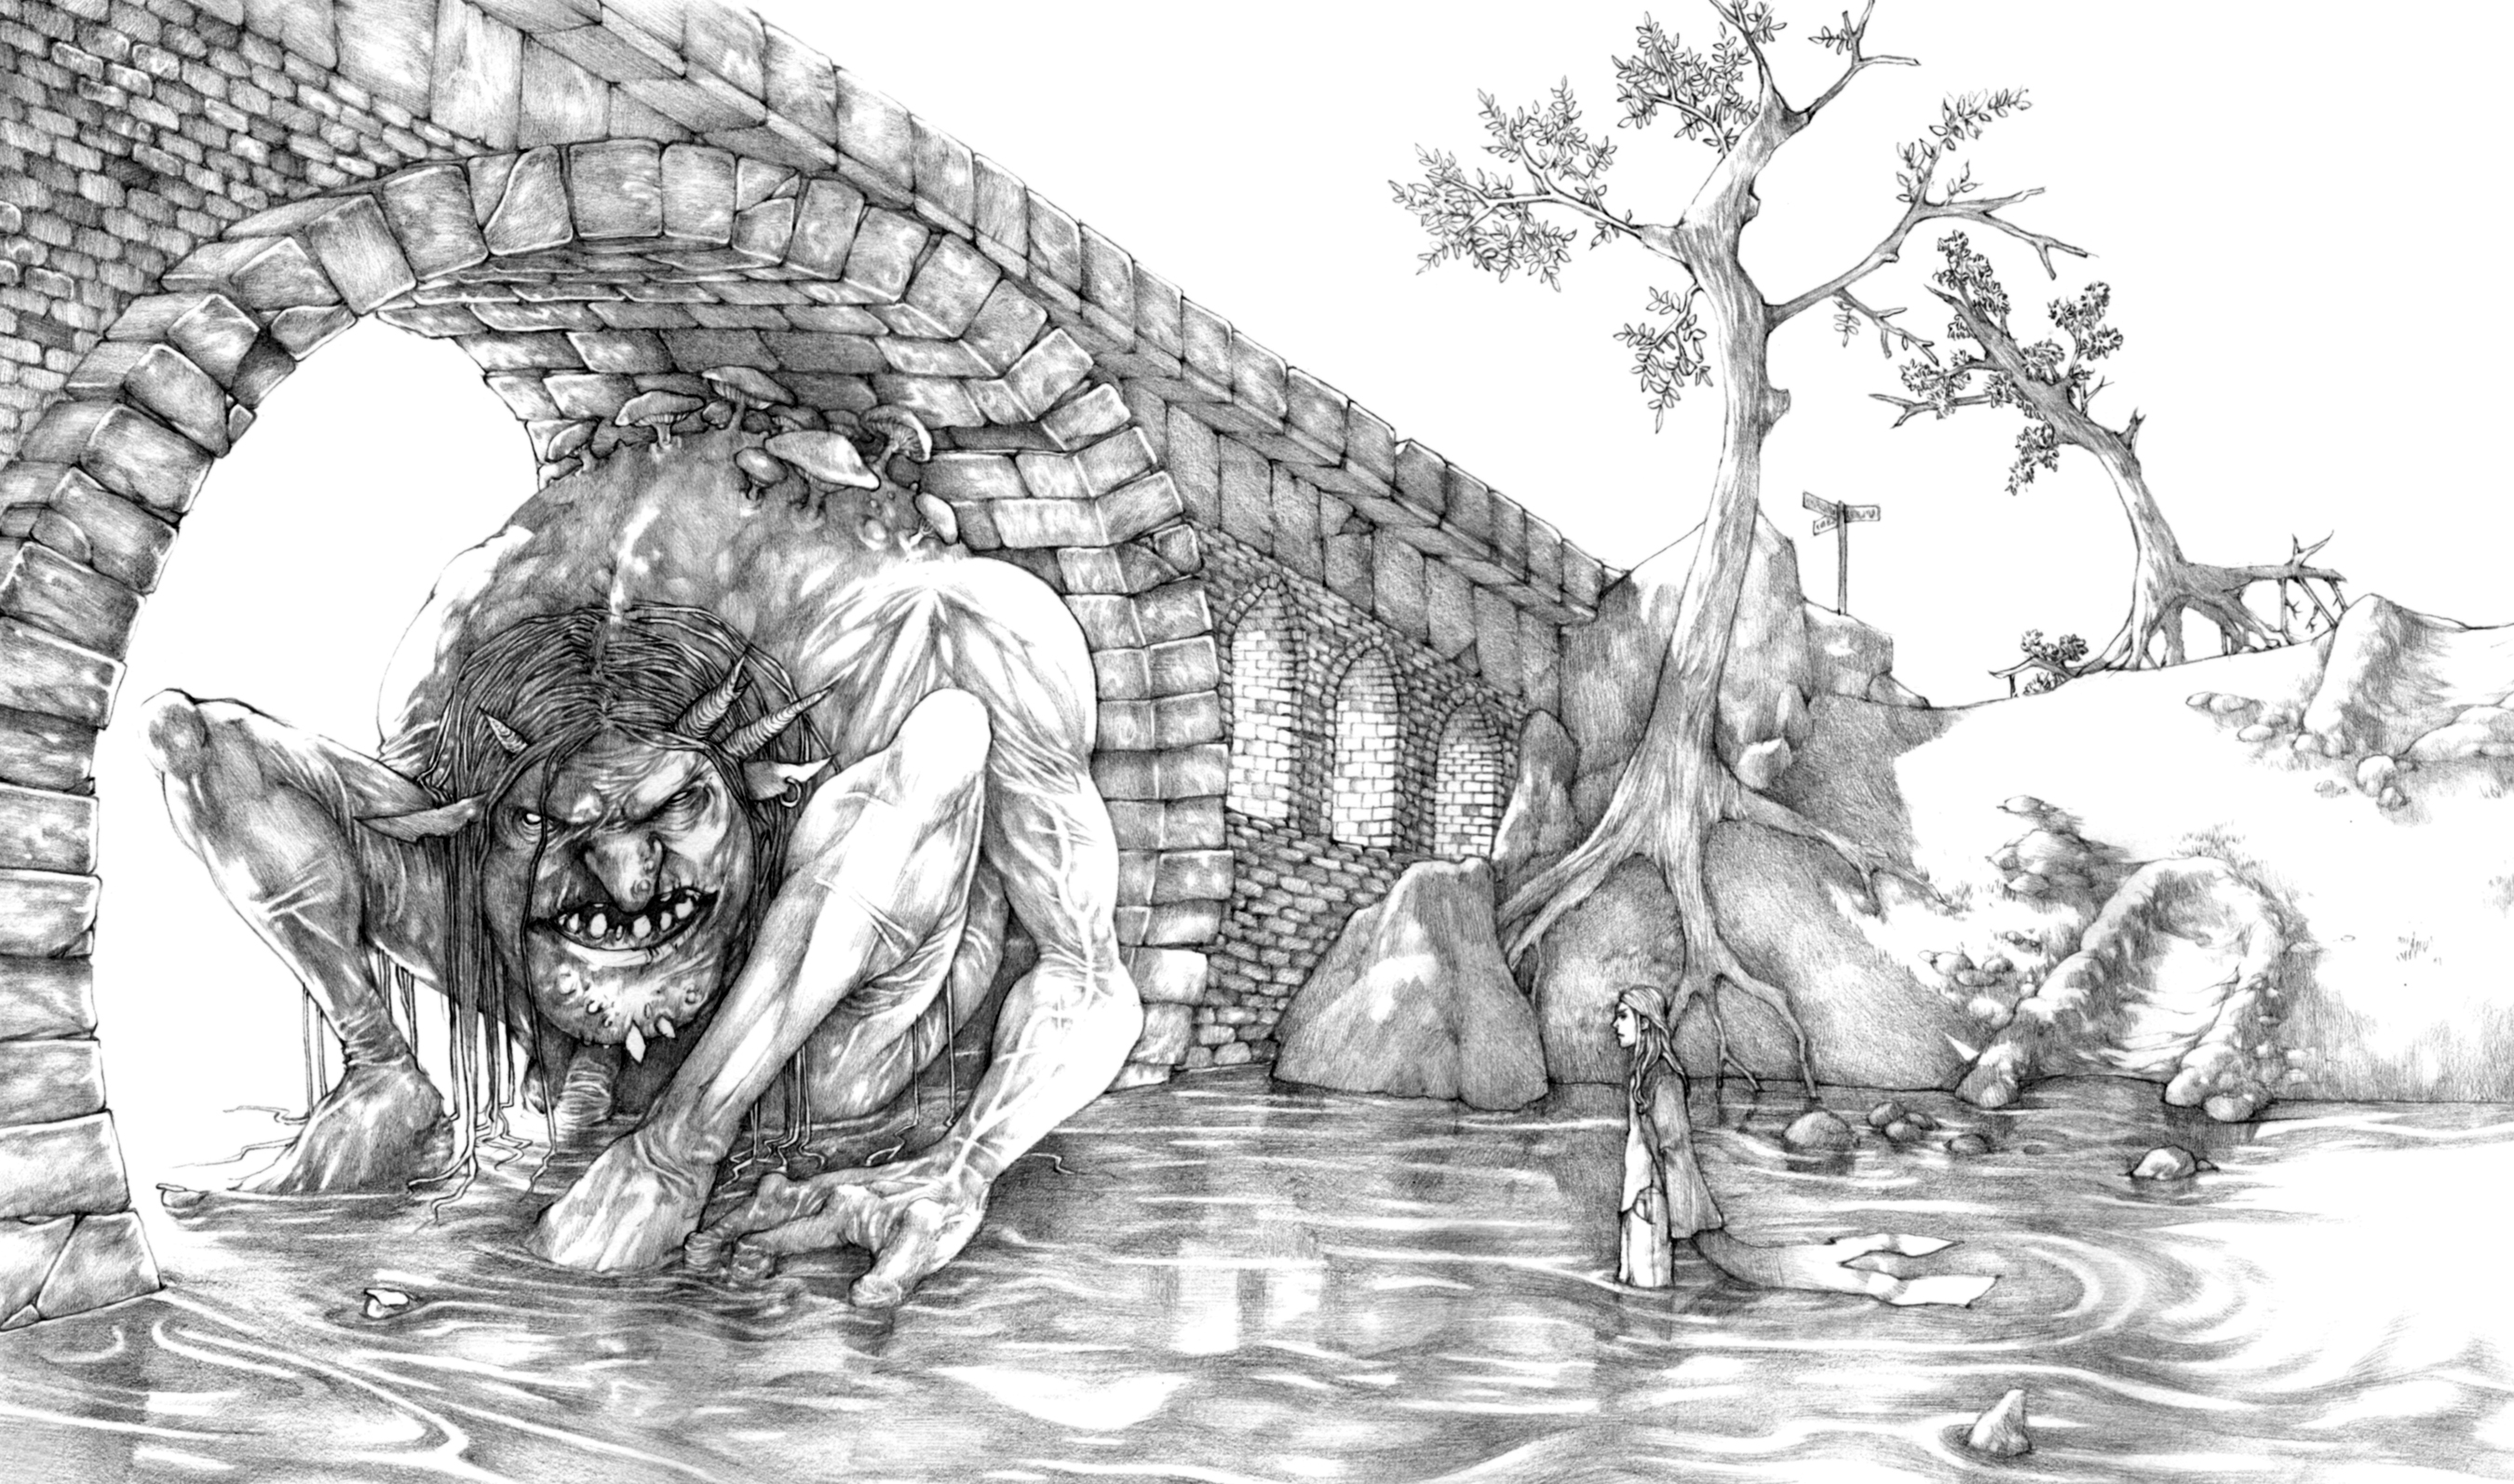
\includegraphics[width=0.8\textwidth]{fig/troll_bridge___pencils_by_gido_d60evd5.jpg}
\end{center}
\begin{flushright}
{\tiny
Illustrated by Gido
}
\end{flushright}
\end{frame}



\begin{frame}\frametitle{Deterministic unary oritatami systems at delay 1}
\begin{block}{Tunnel Troll Theorem}
\begin{description}
	\item[$\alpha \geq 4$] \# of free hands does not increase / tunnel section.
	\item[$\alpha = 3$] Troll consumes bonds / tunnel section.
	\item[$\alpha = 2$] Troll consumes bonds / tunnel.
\end{description}
\end{block}
\begin{columns}[c]
	\begin{column}{0.48\textwidth}
	\begin{tikzpicture}
          \begin{scope}[yshift=2cm]
          
            \draw[white] (60:1) -- (0:0);
            \draw[white] (-60:1) -- (0:0);
            
            \foreach \theta in {60,-60,120,-120}{
              \fill[transform canvas={shift=(\theta:1)}, red](0,0) circle [radius=0.1];
            }
	            \fill(0,0) circle [radius=0.05];
                 \fill[transform canvas={shift=(180:1)}](0,0) circle [radius=0.05];
         	      \fill[blue, transform canvas={shift=(0:1)}](0,0) circle [radius=0.05];
	          \draw[->] (-0.9, 0) -- (-0.1, 0);
	          \draw[->, blue] (0.1, 0) -- (0.9, 0);
	          
		 \node[anchor=center, inner sep=0)] at (-60:1) {
 		   
\includegraphics[width=0.17\textwidth]{fig/TrollFace.jpg}
		 };
          \end{scope}
          

          \node at (0,0) {Tunnel section};
        \end{tikzpicture}
	\end{column}
	
	\begin{column}{0.48\textwidth}
	\begin{tikzpicture}
		\fill[red] (60:1) circle [radius=0.1];
		\fill[red] (-60:1) circle [radius=0.1];
		\fill[red] (120:1) circle [radius=0.1];
		\fill[red] (-120:1) circle [radius=0.1];
		\fill[red, shift=(0:1)] (60:1) circle [radius=0.1];
		\fill[red, shift=(0:1)] (-60:1) circle [radius=0.1];
	
		\fill[shift=(0:-1)] (-120:1) circle [radius=0.05];
		\fill[shift=(0:-1)] (0:0) circle [radius=0.05];
		\draw[shift=(0:-1), ->] (-120:0.9) -- (-120:0.1);
		
		\draw[blue, ->] (180:0.9) -- (180:0.1);
		\fill[blue] (0:0) circle [radius=0.05];
		\draw[blue, ->] (0:0.1) -- (0:0.9);
		\fill[blue] (0:1) circle [radius=0.05];
		
		\fill[blue, shift=(0:2)] (0:0) circle [radius=0.05];
		\draw[blue, shift=(0:2), ->] (180:0.9) -- (180:0.1);
		\draw[blue, shift=(0:2), ->] (60:0.1) -- (60:0.9);
		
		\node at (-90:2) {Tunnel};
		
		\node[anchor=center, inner sep=0, shift=(0:-1)] at (60:1) {
 		   
\includegraphics[width=0.17\textwidth]{fig/TrollFace.jpg}
		 };
	\end{tikzpicture}
	\end{column}
	\end{columns}
\end{frame}

%%%%%
%%%             a = 4           %%%

\begin{frame}\frametitle{Deterministic unary oritatami systems at delay 1}
\begin{block}{Tunnel Troll Theorem}
\begin{description}
	\item[$\alpha \geq 4$] Any hands are not supplied with using a tunnel section.
\end{description}
\end{block}
\begin{center}
\begin{columns}[c]
	\begin{column}{0.48\textwidth}
	\begin{tikzpicture}
		\draw[white] (60:1) -- (0:0);
              \draw[white] (-60:1) -- (0:0);
            
              \foreach \theta in {60,-60,120,-120}{
                 \fill[transform canvas={shift=(\theta:1.5)}, red](0,0) circle [radius=0.1];
               }
	            \fill(0,0) circle [radius=0.05];
                 \fill[transform canvas={shift=(180:1.5)}, red](0,0) circle [radius=0.1];
         	      \fill[blue, transform canvas={shift=(0:1.5)}](0,0) circle [radius=0.05];
	          \draw[->] (-1.3, 0) -- (-0.2, 0);
	          \draw[->, blue] (0.2, 0) -- (1.3, 0);
	          \draw[->, blue, shift=(0:1.5)] (60:0.2) -- (60:1.3);
	          \draw[olive, shift=(0:1.5)] (0:1.5) circle [radius=0.1];
	          \draw[olive, shift=(0:1.5)] (-60:1.5) circle [radius=0.1];
	          
	          \foreach \tta in {0,-60}{
	          \node[anchor=south, inner sep=0, shift=(0:1.5), rotate=(\tta - 90)] at (\tta:0.3) {
 			   
\includegraphics[width=0.08\textwidth]{fig/te.png}
			};
	          }
	          
	          \visible<2>{
%	          \draw[dotted, thick, shift=(0:1)] (120:0.9) -- (120:0.1);
%	          \draw[dotted, thick, shift=(0:1)] (-120:0.9) -- (-120:0.1);
	          \foreach \tta in {120,-120}{
	   	       \node[anchor=west, inner sep=0, shift=(0:1.5), rotate=(\tta - 90)] at (\tta + 10:0.75) {
 				   
\includegraphics[width=0.08\textwidth]{fig/akusyu1.png}
			};
	          }
	     	     \node[anchor=center ,inner sep=0] at (60:1.5) {
 			   
\includegraphics[width=0.17\textwidth]{fig/TrollFace.jpg}
			 };
			 \node[anchor=center, inner sep=0] at (-60:1.5) {
 			   
\includegraphics[width=0.17\textwidth]{fig/TrollFace.jpg}
			 };

			\node at (0,-2) {free hands $\leq 0$};
	          }
	\end{tikzpicture}
	\end{column}
		
	\begin{column}{0.3\textwidth}
	\begin{tikzpicture}
		\foreach \tta in {-120,-60} {
			\fill(\tta:1.5) circle [radius=0.05];
		}
		\foreach \tta in {60, 120,180} {
			\fill[red](\tta:1.5) circle [radius=0.1];
		}
		\foreach \tta in {60,120,180} {
			\node[anchor=west, inner sep=0, rotate=(\tta - 90)] at (\tta + 10:0.75) {
 			   
\includegraphics[width=0.14\textwidth]{fig/akusyu1.png}
			 };
%		 \draw[dotted, thick] (\tta:1.3) -- (\tta:0.2);
		}
		\foreach \tta in {0} {
			\node[anchor=west, inner sep=0, rotate=(\tta - 90)] at (\tta + 10:0.75) {
 			   
\includegraphics[width=0.14\textwidth]{fig/te.png}
			 };
		}
		\fill[blue] (0:0) circle [radius=0.1];
		\draw[->] (-120:1.3) -- (-120:0.2);
		\draw[->] (-60:0.2) -- (-60:1.3);
		
		\draw[olive] (0:1.5) circle [radius=0.1];
	\end{tikzpicture}
	\end{column}
\end{columns}
\end{center}
\end{frame}

%%%%%
%%%             a = 3           %%%

\begin{frame}\frametitle{Deterministic unary oritatami systems at delay 1}
\begin{block}{Tunnel Troll Theorem}
\begin{description}
	\item[$\alpha = 3$] At least one free hand is decreased / tunnel section.
\end{description}
\end{block}

\begin{center}
\begin{columns}[c]
	\begin{column}{0.48\textwidth}
	\begin{tikzpicture}
		\draw[white] (60:1) -- (0:0);
              \draw[white] (-60:1) -- (0:0);
            
              \foreach \theta in {60,-60,120,-120}{
                 \fill[transform canvas={shift=(\theta:1.5)}, red](0,0) circle [radius=0.1];
               }
	            \fill(0,0) circle [radius=0.05];
                 \fill[transform canvas={shift=(180:1.5)}, red](0,0) circle [radius=0.1];
         	      \fill[blue, transform canvas={shift=(0:1.5)}](0,0) circle [radius=0.05];
	          \draw[->] (-1.3, 0) -- (-0.2, 0);
	          \draw[->, blue] (0.2, 0) -- (1.3, 0);
	          \draw[olive, shift=(0:1.5)] (60:1.5) circle [radius=0.1];
	          \draw[olive, shift=(0:1.5)] (-60:1.5) circle [radius=0.1];
	          
	          \visible<1>{
	          \foreach \tta in {0,-60,60}{
	          \node[anchor=south, inner sep=0, shift=(0:1.5), rotate=(\tta - 90)] at (\tta:0.3) {
 			   
\includegraphics[width=0.08\textwidth]{fig/te.png}
			};
	          }
	          }
	          
	          \visible<2>{
	          \foreach \tta in {120,-120}{
	   	       \node[anchor=west, inner sep=0, shift=(0:1.5), rotate=(\tta - 90)] at (\tta + 10:0.75) {
 				   
\includegraphics[width=0.08\textwidth]{fig/akusyu1.png}
			};
	          }
	           \node[anchor=south, inner sep=0, shift=(0:1.5), rotate=-90] at (0:0.3) {
 			   
\includegraphics[width=0.08\textwidth]{fig/te.png}
			};
	     	     \node[anchor=center ,inner sep=0] at (60:1.5) {
 			   
\includegraphics[width=0.17\textwidth]{fig/TrollFace.jpg}
			 };
			 \node[anchor=center, inner sep=0] at (-60:1.5) {
 			   
\includegraphics[width=0.17\textwidth]{fig/TrollFace.jpg}
			 };

			
	      		    \node at (-0.1,-2.6) {free hands $\leq -1$};
	          }
	          

	          \visible<3>{
	          \foreach \tta in {60,-120}{
	   	       \node[anchor=west, inner sep=0, shift=(0:1.5), rotate=(\tta - 90)] at (\tta + 10:0.75) {
 				   
\includegraphics[width=0.08\textwidth]{fig/akusyu1.png}
			};
	          }
	     	     \node[anchor=center ,inner sep=0, shift=(0:1.5)] at (60:1.5) {
 			   
\includegraphics[width=0.17\textwidth]{fig/TrollFace.jpg}
			 };
			 \node[anchor=center, inner sep=0] at (-60:1.5) {
 			   
\includegraphics[width=0.17\textwidth]{fig/TrollFace.jpg}
			 };
	           \node[anchor=south, inner sep=0, shift=(0:1.5), rotate=-150] at (-60:0.3) {
 			   
\includegraphics[width=0.08\textwidth]{fig/te.png}
			};
			\draw[olive, shift=(0:1.5)] (0:1.5) circle [radius=0.1];
	      		    \node at (-0.1,-2.6) {free hands $\leq -1$};
	          }
	           \visible<4>{
	           	\foreach \tta in {60,0,-60}{
				\fill[red, shift=(0:1.5)] (\tta:1.5) circle [radius=0.1];
			}
			 \node at (0,-2) {terminal conformaion};
	          }
	\end{tikzpicture}
	\end{column}
		
	\begin{column}{0.3\textwidth}
	\begin{tikzpicture}
		\foreach \tta in {-120,-60} {
			\fill(\tta:1.5) circle [radius=0.05];
		}
		\foreach \tta in {120,180} {
			\fill[red](\tta:1.5) circle [radius=0.1];
		}
		\foreach \tta in {120,180} {
			\node[anchor=west, inner sep=0, rotate=(\tta - 90)] at (\tta + 10:0.75) {
 			   
\includegraphics[width=0.14\textwidth]{fig/akusyu1.png}
			 };
		}
		\foreach \tta in {60} {
			\node[anchor=west, inner sep=0, rotate=(\tta - 90)] at (\tta + 10:0.75) {
 			   
\includegraphics[width=0.14\textwidth]{fig/te.png}
			 };
		}
		\fill[blue] (0:0) circle [radius=0.1];
		\draw[->] (-120:1.3) -- (-120:0.2);
		\draw[->] (-60:0.2) -- (-60:1.3);
		
		\draw[olive] (0:1.5) circle [radius=0.1];
		\draw[olive] (60:1.5) circle [radius=0.1];
	\end{tikzpicture}
	\end{column}
\end{columns}
\end{center}

%\begin{columns}[c]
%	\begin{column}{0.48\textwidth}
%	\begin{tikzpicture}
%		\draw[white] (60:1) -- (0:0);
%              \draw[white] (-60:1) -- (0:0);
%            
%              \foreach \theta in {60,-60,120,-120}{
%                 \fill[transform canvas={shift=(\theta:1)}, red](0,0) circle [radius=0.1];
%               }
%	            \fill(0,0) circle [radius=0.05];
%                 \fill[transform canvas={shift=(180:1)}, red](0,0) circle [radius=0.1];
%         	      \fill[blue, transform canvas={shift=(0:1)}](0,0) circle [radius=0.05];
%	          \draw[->] (-0.9, 0) -- (-0.1, 0);
%	          \draw[->, blue] (0.1, 0) -- (0.9, 0);
%	          \draw[olive, shift=(0:1)] (60:1) circle [radius=0.1];
%	          \draw[olive, shift=(0:1)] (-60:1) circle [radius=0.1];
%	          
%	          \visible<2>{
%	          \draw[dotted, thick, shift=(0:1)] (120:0.9) -- (120:0.1);
%	          \draw[dotted, thick, shift=(0:1)] (-120:0.9) -- (-120:0.1);
%	     	     \node[anchor=center ,inner sep=0] at (60:1) {
% 			   
\includegraphics[width=0.17\textwidth]{fig/TrollFace.jpg}
%			 };
%			 \node[anchor=center, inner sep=0] at (-60:1) {
% 			   
\includegraphics[width=0.17\textwidth]{fig/TrollFace.jpg}
%			 };
%			\node at (-0.1,-2.6) {free hands $\leq -1$};
%	          }
%	          \visible<3>{
%	          \draw[dotted, thick, shift=(0:1)] (60:0.9) -- (60:0.1);
%	          \draw[dotted, thick, shift=(0:1)] (-120:0.9) -- (-120:0.1);
%	     	     \node[anchor=center ,inner sep=0, shift=(0:1)] at (60:1) {
% 			   
\includegraphics[width=0.17\textwidth]{fig/TrollFace.jpg}
%			 };
%			 \node[anchor=center, inner sep=0] at (-60:1) {
% 			   
\includegraphics[width=0.17\textwidth]{fig/TrollFace.jpg}
%			 };
%			\draw[olive, shift=(0:1)] (0:1) circle [radius=0.1];
%	      		    \node at (-0.1,-2.6) {free hands $\leq -1$};
%	          }
%	           \visible<4>{
%	           	\foreach \tta in {60,0,-60}{
%				\fill[red, shift=(0:1)] (\tta:1) circle [radius=0.1];
%			}
%			 \node at (0,-2) {terminal conformaion};
%	          }
%	\end{tikzpicture}
%	\end{column}
%		
%	\begin{column}{0.3\textwidth}
%	\begin{tikzpicture}
%		\foreach \tta in {60,120,180,-120,-60} {
%			\fill(\tta:1) circle [radius=0.05];
%		}
%		\foreach \tta in {60,120,180} {
%		 \draw[dotted, thick] (\tta:0.9) -- (\tta:0.2);
%		}
%		\fill[red] (0:0) circle [radius=0.1];
%		\draw[olive] (0:1) circle [radius=0.1];
%		\draw[->] (-120:0.9) -- (-120:0.2);
%		\draw[->] (-60:0.2) -- (-60:0.9);
%	\end{tikzpicture}
%	\end{column}
%\end{columns}

\end{frame}

%%%%%
%%%             a = 2           %%%

\begin{frame}\frametitle{Deterministic unary oritatami systems at delay 1}
\begin{block}{Tunnel Troll Theorem}
\begin{description}
	\item[$\alpha = 2$] At least one free hand is decreased / tunnel.
\end{description}
\end{block}

\begin{columns}[c]
	\begin{column}{0.48\textwidth}
	\begin{tikzpicture}
\draw[white] (60:1) -- (0:0);
              \draw[white] (-60:1) -- (0:0);
            
              \foreach \theta in {60,-60,120,-120}{
                 \fill[transform canvas={shift=(\theta:1.5)}, red](0,0) circle [radius=0.1];
               }
	            \fill(0,0) circle [radius=0.05];
                 \fill[transform canvas={shift=(180:1.5)}, red](0,0) circle [radius=0.1];
	          \draw[olive, shift=(0:1.5)] (60:1.5) circle [radius=0.1];
	          \draw[olive, shift=(0:1.5)] (-60:1.5) circle [radius=0.1];
	          
	          \invisible<2>{
	          	 \draw[->] (-1.3, 0) -- (-0.2, 0);
	          	 \draw[->, blue] (0.2, 0) -- (1.3, 0);
	 		\fill[blue, transform canvas={shift=(0:1.5)}](0,0) circle [radius=0.05];
	          }
	          
	          \visible<1,3>{
	          \foreach \tta in {-60,60}{
	          \node[anchor=south, inner sep=0, shift=(0:1.5), rotate=(\tta - 90)] at (\tta:0.3) {
 			   
\includegraphics[width=0.08\textwidth]{fig/te.png}
			};
	          }
	          }
%        	\invisible<2>{
%			 \fill[blue, transform canvas={shift=(0:1)}](0,0) circle [radius=0.05];
%			\fill(0,0) circle [radius=0.05];
%	          \draw[->] (-0.9, 0) -- (-0.1, 0);
%	          \draw[->, blue] (0.1, 0) -- (0.9, 0);
%	       }
	       \visible<2>{
			\fill[blue](0,0) circle [radius=0.05];
	          \draw[->, blue] (-1.3, 0) -- (-0.2, 0);
	          \draw[olive] (0:1.5) circle [radius=0.1];
	       }

	          \visible<3>{
	          \foreach \tta in {60,-60}{
	   	       \node[anchor=west, inner sep=0, rotate=(\tta - 90)] at (\tta + 10:0.75) {
 				   
\includegraphics[width=0.08\textwidth]{fig/akusyu1.png}
			};
	          }
	     	     \node[anchor=center ,inner sep=0] at (60:1.5) {
 			   
\includegraphics[width=0.17\textwidth]{fig/TrollFace.jpg}
			 };
			 \node[anchor=center, inner sep=0] at (-60:1.5) {
 			   
\includegraphics[width=0.17\textwidth]{fig/TrollFace.jpg}
			 };
	      		    \node at (0,-2) {free hands $\leq 0$};
	          }
	          \visible<4>{
	          \foreach \tta in {-60}{
	          \node[anchor=south, inner sep=0, shift=(0:1.5), rotate=(\tta - 90)] at (\tta:0.3) {
 			   
\includegraphics[width=0.08\textwidth]{fig/te.png}
			};
	          }
	          \foreach \tta in {-60}{
	   	       \node[anchor=west, inner sep=0, rotate=(\tta - 90)] at (\tta + 10:0.75) {
 				   
\includegraphics[width=0.08\textwidth]{fig/akusyu1.png}
			};
	          }
	          \fill[red, shift=(0:1.5)] (60:1.5) circle [radius=0.1];
			 \node[anchor=center, inner sep=0] at (-60:1.5) {
 			   
\includegraphics[width=0.17\textwidth]{fig/TrollFace.jpg}
			 };
			 \node at (0,-2) {free hands $\leq 0$};
	          }
	           \visible<5>{
	           	\foreach \tta in {60,-60}{
				\fill[red, shift=(0:1.5)] (\tta:1.5) circle [radius=0.1];
			}
			\draw[olive, shift=(0:1.5)] (0:1.5) circle [radius=0.1];
			 \node at (0,-2) {inside tunnel};
	          }
	\end{tikzpicture}
	\end{column}
		
	\begin{column}{0.3\textwidth}
	\begin{tikzpicture}
		\foreach \tta in {-120,-60} {
			\fill(\tta:1.5) circle [radius=0.05];
		}
		\foreach \tta in {180} {
			\fill[red](\tta:1.5) circle [radius=0.1];
		}
		\foreach \tta in {180} {
			\node[anchor=west, inner sep=0, rotate=(\tta - 90)] at (\tta + 10:0.75) {
 			   
\includegraphics[width=0.14\textwidth]{fig/akusyu1.png}
			 };
		}
		\foreach \tta in {120} {
			\node[anchor=west, inner sep=0, rotate=(\tta - 90)] at (\tta + 10:0.75) {
 			   
\includegraphics[width=0.14\textwidth]{fig/te.png}
			 };
		}
		\fill[blue] (0:0) circle [radius=0.1];
		\draw[->] (-120:1.3) -- (-120:0.2);
		\draw[->] (-60:0.2) -- (-60:1.3);
		
		\draw[olive] (0:1.5) circle [radius=0.1];
		\draw[olive] (60:1.5) circle [radius=0.1];
		\draw[olive] (120:1.5) circle [radius=0.1];
	\end{tikzpicture}
	\end{column}
\end{columns}

\end{frame}


%%%%%%%%%%%%%
%%% entrance

\begin{frame}\frametitle{Deterministic unary oritatami systems at delay 1}
  \begin{block}{Jordan curve theorem}
    A closed curve which is a non-self-intersecting divides into inside and outside.
  \end{block}

  \begin{center}
\begin{columns}[c]
\begin{column}{0.4\textwidth}
        \begin{tikzpicture}
		\fill[teal!20] (60:1) 
					to[out=150, in=-20] (120: 1.5)
		                    to[out=160, in=90] (180:1.9)
		                    to[out=-90, in=-160] (-160:1.4)
		                    to[out=20, in=-150] (-60:1)
		                    -- (0:1) -- (60:1) -- cycle;
		
        	\draw[teal] (60:1) 
					to[out=150, in=-20] (120: 1.5)
		                    to[out=160, in=90] (180:1.9)
		                    to[out=-90, in=-160] (-160:1.4)
		                    to[out=20, in=-150] (-60:1);
		
        	\fill[red, shift=(0:1)] (60:1) circle [radius=0.1];
		\fill[red, shift=(0:1)] (-60:1) circle [radius=0.1];
        	\fill[red] (60:1) circle [radius=0.1];
		\fill[red] (-60:1) circle [radius=0.1];
		\draw[->] (0:0) -- (0:0.9);
		\fill[orange] (0:0) circle [radius=0.07];
		\draw (0:1) circle [radius=0.05];
		\draw (0:2) circle [radius=0.05];
		
		\draw[dotted, thick] (60:0.1) -- (60:0.9);
		
		\draw[->] (120:0.85) -- (120:0.1);
		
		\node[anchor=south, inner sep=0, rotate=(-120 - 90)] at (-120:0.2) {
 			   
\includegraphics[width=0.1\textwidth]{fig/te.png}
		};
		
        \end{tikzpicture}
        
    \end{column}
    
    \begin{column}{0.4\textwidth}
        \begin{tikzpicture}
        

    \fill[teal!20] (60:1) 
					to[out=60, in=110] (40: 2.4)
		                    to[out=-70, in=90] (0:3.2)
		                    to[out=-90, in=60] (-20:2.4)
		                    to[out=-120, in=-40] (-60:1)
		                    -- (0:1) -- (60:1) -- cycle;
		
        	\draw[teal] (60:1) 
					to[out=60, in=110] (40: 2.4)
		                    to[out=-70, in=90] (0:3.2)
		                    to[out=-90, in=60] (-20:2.4)
		                    to[out=-120, in=-40] (-60:1);
		
        	\fill[red, shift=(0:1)] (60:1) circle [radius=0.1];
		\fill[red, shift=(0:1)] (-60:1) circle [radius=0.1];
        	\fill[red] (60:1) circle [radius=0.1];
		\fill[red] (-60:1) circle [radius=0.1];
		\draw[->] (0:0) -- (0:0.9);
		\fill[orange] (0:0) circle [radius=0.07];
		\draw (0:1) circle [radius=0.05];
		\draw (0:2) circle [radius=0.05];
		
		\draw[->] (120:0.85) -- (120:0.1);
		
		
		\draw[dotted, thick] (60:0.1) -- (60:0.9);		
		
		\node[anchor=south, inner sep=0, rotate=(-120 - 90)] at (-120:0.2) {
 			   
\includegraphics[width=0.1\textwidth]{fig/te.png}
		};
        \end{tikzpicture}
        
    \end{column}

\end{columns}


At $\alpha = 2$, Troll consumes free hands an entrance of tunnel, too.

\end{center}
\end{frame}



\begin{frame}

\begin{center}
{ \fontsize{30pt}{4pt}\selectfont
Thank you for listening!!
}
\end{center}

\end{frame}





%%%%%%%%%%%%%%%%
%%%%%%%%%%%%%%%%%%%



%%%%%%%%%%%%%%%%%%%
%%%%%%%%%%%%%               a = 2 entrance of tunnel

\begin{frame}\frametitle{Deterministic unary oritatami systems at delay 1}
  \begin{block}{Tunnel Troll Theorem ($\alpha = 2$)}
    Type of tunnel sections
  \end{block}

      
  \begin{columns}[c]
    \begin{column}{0.3\textwidth}   
%    	\begin{figure}
        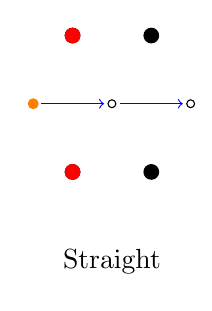
\begin{tikzpicture}
          \begin{scope}[xshift=2cm, yshift=2cm]
          
            \draw[white] (60:1) -- (0:0);
            \draw[white] (-60:1) -- (0:0);
            \draw(0,0) circle [radius=0.05];

            \foreach \theta in {0,180}{
              \draw[transform canvas={shift=(\theta:1)}](0,0) circle [radius=0.05];
            }
            
            \foreach \theta in {60,-60,120,-120}{
              \fill[transform canvas={shift=(\theta:1)}](0,0) circle [radius=0.1];
            }
          \draw[->, blue] (-0.9, 0) -- (-0.1, 0);
          \draw[->, blue] (0.1, 0) -- (0.9, 0);
          
          \visible<2>{
          	\fill[red] (120:1) circle [radius=0.1];
		\fill[red] (-120:1) circle [radius=0.1];
		\fill[orange] (180:1) circle [radius=0.07];
          }
          \end{scope}
          

          \node at (2,0) {Straight};
        \end{tikzpicture}
%      \end{figure}
    \end{column}
    
    \begin{column}{0.3\textwidth}
        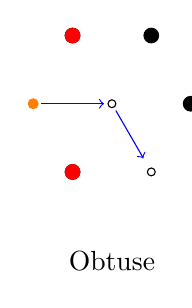
\begin{tikzpicture}

          \begin{scope}[xshift=2cm, yshift=2cm]
          
            \draw[white] (60:1) -- (0:0);
            \draw[white] (-60:1) -- (0:0);
            \draw(0,0) circle [radius=0.05];

            \foreach \theta in {-60,180}{
              \draw[transform canvas={shift=(\theta:1)}](0,0) circle [radius=0.05];
            }
            
            \foreach \theta in {0,60,120,-120}{
 	            \fill[transform canvas={shift=(\theta:1)}](0,0) circle [radius=0.1];
            }
          \draw[->, blue] (-0.9, 0) -- (-0.1, 0);
          \draw[->, blue] (0,0)++(300:0.1) -- (300:0.8);
          \visible<2>{
          	\fill[red] (120:1) circle [radius=0.1];
		\fill[red] (-120:1) circle [radius=0.1];
		\fill[orange] (180:1) circle [radius=0.07];
          }
          \end{scope}

          \node at (2,0) {Obtuse};
        \end{tikzpicture}
        
    \end{column}

    \begin{column}{0.3\textwidth}
        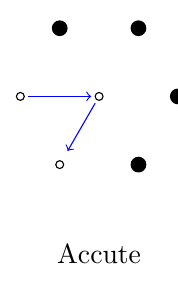
\begin{tikzpicture}

          \begin{scope}[xshift=2cm, yshift=2cm]
            \draw[white] (60:1) -- (0:0);
            \draw[white] (-60:1) -- (0:0);
            \draw(0,0) circle [radius=0.05];

            \foreach \theta in {-120,180}{
              \draw[transform canvas={shift=(\theta:1)}](0,0) circle [radius=0.05];
            }
            
            \foreach \theta in {0,60,-60,120}{
              \fill[transform canvas={shift=(\theta:1)}](0,0) circle [radius=0.1];
            }
          \draw[->, blue] (-0.9, 0) -- (-0.1, 0);
          \draw[->, blue] (0,0)++(240:0.1) -- (240:0.8);
          \end{scope}

          \node at (2,0) {Accute};
        \end{tikzpicture}
    \end{column}
  \end{columns}
\end{frame}


%%%%%%%%%%%

\begin{frame}\frametitle{Deterministic unary oritatami systems at delay 1}
  \begin{block}{Tunnel Troll Theorem ($\alpha = 2$)}
    Directions to enter a tunnel
  \end{block}

      
  \begin{columns}[c]
    \begin{column}{0.3\textwidth}   
%    	\begin{figure}
        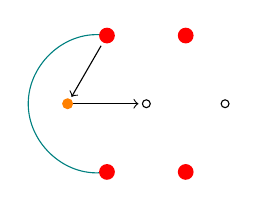
\begin{tikzpicture}
        	\visible<2>{
        	\draw[teal] (60:1) 
		                    to[out=170, in=90] (180:0.5)
		                    to[out=-90, in=-170] (-60:1);
		}
        	\fill[red, shift=(0:1)] (60:1) circle [radius=0.1];
		\fill[red, shift=(0:1)] (-60:1) circle [radius=0.1];
        	\fill[red] (60:1) circle [radius=0.1];
		\fill[red] (-60:1) circle [radius=0.1];
		\draw[->] (0:0) -- (0:0.9);
		\fill[orange] (0:0) circle [radius=0.07];
		\draw (0:1) circle [radius=0.05];
		\draw (0:2) circle [radius=0.05];
		
		\draw[->] (60:0.85) -- (60:0.1);
        \end{tikzpicture}
%      \end{figure}
    \end{column}
    
    \begin{column}{0.3\textwidth}
        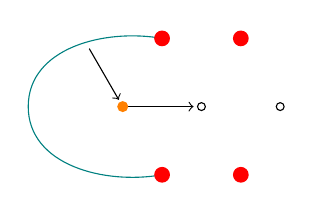
\begin{tikzpicture}
        	\visible<2>{
        	\draw[teal] (60:1) 
		                    to[out=170, in=90] (180:1.2)
		                    to[out=-90, in=-170] (-60:1);
		}
        	\fill[red, shift=(0:1)] (60:1) circle [radius=0.1];
		\fill[red, shift=(0:1)] (-60:1) circle [radius=0.1];
        	\fill[red] (60:1) circle [radius=0.1];
		\fill[red] (-60:1) circle [radius=0.1];
		\draw[->] (0:0) -- (0:0.9);
		\fill[orange] (0:0) circle [radius=0.07];
		\draw (0:1) circle [radius=0.05];
		\draw (0:2) circle [radius=0.05];
		
		\draw[->] (120:0.85) -- (120:0.1);
        \end{tikzpicture}
        
    \end{column}

    \begin{column}{0.3\textwidth}
        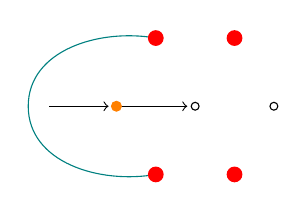
\begin{tikzpicture}
        	\visible<2>{
        	\draw[teal] (60:1) 
		                    to[out=170, in=90] (180:1.12)
		                    to[out=-90, in=-170] (-60:1);
		}
        	\fill[red, shift=(0:1)] (60:1) circle [radius=0.1];
		\fill[red, shift=(0:1)] (-60:1) circle [radius=0.1];
        	\fill[red] (60:1) circle [radius=0.1];
		\fill[red] (-60:1) circle [radius=0.1];
		\draw[->] (0:0) -- (0:0.9);
		\fill[orange] (0:0) circle [radius=0.07];
		\draw (0:1) circle [radius=0.05];
		\draw (0:2) circle [radius=0.05];
		
		\draw[->] (180:0.85) -- (180:0.1);
	 \end{tikzpicture}
    \end{column}
  \end{columns}
  \begin{center}
  	\visible<2>{
	  	freehands $\leq \pm 0$
	}
	
	

\visible<2>{
	
\begin{columns}[c]
\begin{column}{0.4\textwidth}
        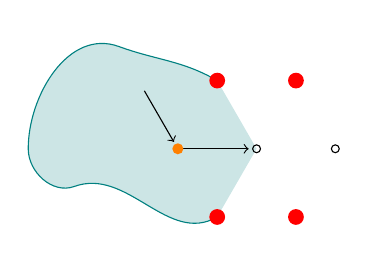
\begin{tikzpicture}
		\fill[teal!20] (60:1) 
					to[out=150, in=-20] (120: 1.5)
		                    to[out=160, in=90] (180:1.9)
		                    to[out=-90, in=-160] (-160:1.4)
		                    to[out=20, in=-150] (-60:1)
		                    -- (0:1) -- (60:1) -- cycle;
		
        	\draw[teal] (60:1) 
					to[out=150, in=-20] (120: 1.5)
		                    to[out=160, in=90] (180:1.9)
		                    to[out=-90, in=-160] (-160:1.4)
		                    to[out=20, in=-150] (-60:1);
		
        	\fill[red, shift=(0:1)] (60:1) circle [radius=0.1];
		\fill[red, shift=(0:1)] (-60:1) circle [radius=0.1];
        	\fill[red] (60:1) circle [radius=0.1];
		\fill[red] (-60:1) circle [radius=0.1];
		\draw[->] (0:0) -- (0:0.9);
		\fill[orange] (0:0) circle [radius=0.07];
		\draw (0:1) circle [radius=0.05];
		\draw (0:2) circle [radius=0.05];
		
		\draw[->] (120:0.85) -- (120:0.1);
		
		
        \end{tikzpicture}
        
    \end{column}
    
    \begin{column}{0.4\textwidth}
        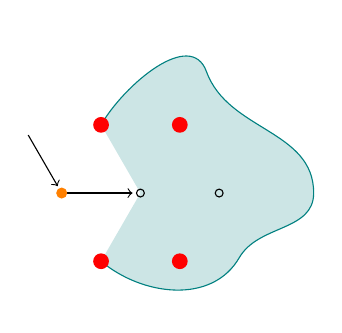
\begin{tikzpicture}
        

    \fill[teal!20] (60:1) 
					to[out=60, in=110] (40: 2.4)
		                    to[out=-70, in=90] (0:3.2)
		                    to[out=-90, in=60] (-20:2.4)
		                    to[out=-120, in=-40] (-60:1)
		                    -- (0:1) -- (60:1) -- cycle;
		
        	\draw[teal] (60:1) 
					to[out=60, in=110] (40: 2.4)
		                    to[out=-70, in=90] (0:3.2)
		                    to[out=-90, in=60] (-20:2.4)
		                    to[out=-120, in=-40] (-60:1);
		
        	\fill[red, shift=(0:1)] (60:1) circle [radius=0.1];
		\fill[red, shift=(0:1)] (-60:1) circle [radius=0.1];
        	\fill[red] (60:1) circle [radius=0.1];
		\fill[red] (-60:1) circle [radius=0.1];
		\draw[->] (0:0) -- (0:0.9);
		\fill[orange] (0:0) circle [radius=0.07];
		\draw (0:1) circle [radius=0.05];
		\draw (0:2) circle [radius=0.05];
		
		\draw[->] (120:0.85) -- (120:0.1);
        \end{tikzpicture}
        
    \end{column}

\end{columns}

}

\end{center}
\end{frame}

%%%%%%%%%%%%%%
%%%%%           entrance of tunnel section on previous

\begin{frame}\frametitle{Deterministic unary oritatami systems at delay 1}
  \begin{block}{Tunnel Troll Theorem ($\alpha = 2$)}
    If this orange bead is stabilized by bonds, total bonds decrease.
  \end{block}

      
  \begin{columns}[c]
    \begin{column}{0.3\textwidth}   
%    	\begin{figure}
        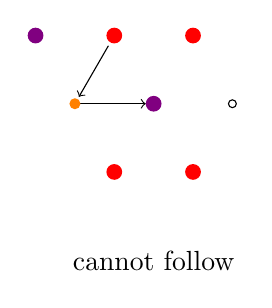
\begin{tikzpicture}
        	\fill[red, shift=(0:1)] (60:1) circle [radius=0.1];
		\fill[red, shift=(0:1)] (-60:1) circle [radius=0.1];
        	\fill[red] (60:1) circle [radius=0.1];
		\fill[red] (-60:1) circle [radius=0.1];
		\draw[->] (0:0) -- (0:0.9);
		\fill[orange] (0:0) circle [radius=0.07];
		\draw (0:1) circle [radius=0.05];
		\draw (0:2) circle [radius=0.05];
		
		\draw[->] (60:0.85) -- (60:0.1);
		
        	\visible<2>{
        		\fill[violet] (0:1) circle [radius=0.1];
			\fill[violet] (120:1) circle [radius=0.1];
			\node at (1,-2) {cannot follow};
		}
        \end{tikzpicture}
%      \end{figure}
    \end{column}
    
    \begin{column}{0.3\textwidth}
        \begin{tikzpicture}
        	\fill[red, shift=(0:1)] (60:1) circle [radius=0.1];
		\fill[red, shift=(0:1)] (-60:1) circle [radius=0.1];
        	\fill[red] (60:1) circle [radius=0.1];
		\fill[red] (-60:1) circle [radius=0.1];
		\draw[->] (0:0) -- (0:0.9);
		\fill[orange] (0:0) circle [radius=0.07];
		\draw (0:1) circle [radius=0.05];
		\draw (0:2) circle [radius=0.05];
		
		\draw[->] (120:0.85) -- (120:0.1);
        	\visible<2>{
        		\fill[violet] (60:1) circle [radius=0.1];
			\fill[violet] (180:1) circle [radius=0.1];
			\draw[olive] (-120:1) circle [radius=0.1];
			\draw[dotted, thick] (-60:0.1) -- (-60:1);
			\node[anchor=center, inner sep=0] at (-60:1) {
 			   
\includegraphics[width=0.25\textwidth]{fig/TrollFace.jpg}
			 };
			\node at (0.5,-2) {Troll...};
		}
        \end{tikzpicture}
        
    \end{column}

    \begin{column}{0.3\textwidth}
        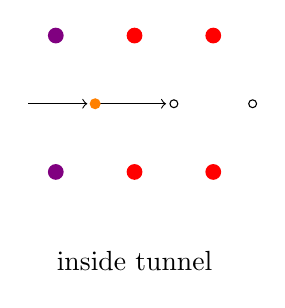
\begin{tikzpicture}
        	\fill[red, shift=(0:1)] (60:1) circle [radius=0.1];
		\fill[red, shift=(0:1)] (-60:1) circle [radius=0.1];
        	\fill[red] (60:1) circle [radius=0.1];
		\fill[red] (-60:1) circle [radius=0.1];
		\draw[->] (0:0) -- (0:0.9);
		\fill[orange] (0:0) circle [radius=0.07];
		\draw (0:1) circle [radius=0.05];
		\draw (0:2) circle [radius=0.05];
		
		\draw[->] (180:0.85) -- (180:0.1);
        	\visible<2>{
        		\fill[violet] (-120:1) circle [radius=0.1];
			\fill[violet] (120:1) circle [radius=0.1];
			\node at (0.5,-2) {inside tunnel};
		}
	 \end{tikzpicture}
    \end{column}
  \end{columns}
  
    \begin{center}
  	\visible<2>{
	  	freehands $\leq -1$\\
	}
\end{center}
\end{frame}


%%%%%%%%%%%%%%%%%%%%%%%%%%%%%%%%%%%%%%%%%%%%%%%%%%%%%%

%%%%%%%%%%%%%%%%%%%%%%%%%%%%%%%%%

\subsection{Upper bound proof}

%%%%%%%  a = 4

%\begin{frame}\frametitle{Deterministic unary oritatami systems at delay 1}
%\begin{block}{$\alpha = 4$}
%The terminal conformation at $\alpha = 4$ is of length at most $3n^2  + 3n + 1$($\hexagon_{O}^n$).
%\end{block}
%
%\begin{center}
%    \begin{tikzpicture}
%
%	\fill (0,0) circle [radius=0.1];
%        \fill[blue] (60:1) circle [radius=0.05];
%        \fill (0:1) circle [radius=0.1];
%        
%	\draw[dotted, thick] (1, 0) -- ++(120:1);
%      
%      \draw[dashed] (180:2) -- (0:2);
%      \draw[dashed, shift=(60:1)] (180:2.5) -- (0:1.5);
%      \draw[->, blue] (60:0.1) -- (60:0.9);
%
%	\node[above] at (180:1) {$p_1$};
%	\node[left] at (-120:1) {$p_2$};
%	\node[left, shift=(-120:1)] at (-60:1) {$p_3$};
%	\node[right] at (-60:1) {$p_4$};
%
%	\draw (180:1) circle [radius=0.05];
%	\draw (-120:1) circle [radius=0.05];
%	\draw (-60:1) circle [radius=0.05];
%	\draw[shift=(-120:1)] (-60:1) circle [radius=0.05];
%
%	\node at (0:2.5) {$n$};
%	\node[shift=(60:1)] at (0:2) {$n+1$};
%    \end{tikzpicture}
%    \end{center}
%\end{frame}

%%%%%%%%%%%%%%%%%%%%%%%%%%%%%%%%%%
%%%%%%%%%%% a = 3

%\begin{frame}\frametitle{Deterministic unary oritatami systems at delay 1}
%\begin{block}{$\alpha = 3$}
%The terminal conformation at $\alpha = 3$ is of length at most $4n + 14$.
%\end{block}
%
%\centering
%
%\scalebox{0.8}{
%	\begin{columns}[c]
%	\begin{column}{0.3\textwidth}
%   \begin{tikzpicture}
%      \node[right, white] at (60:2) {$n_{adj}$};
%      
%      \fill[shift=(180:1)] (0,0) circle [radius=0.1];
%      \fill[shift=(180:0)] (0,0) circle [radius=0.1];
%      
%      \fill[blue](0:1) circle [radius=0.05];
%      
%      \draw[->] (180:0.9) -- (180:0.1);
%      \draw[->, blue] (0:0.1) -- (0:0.9);
%
%	%\node[above] at (180:1) {$w_{[i-2]}$};
%	%\node[below] at (180:0) {$w_{[i-1]}$};
%	\node[above] at (0:1) {$w_{[i]}$};
%
%	\foreach \theta in {60,-60,120,-120}{
%   	   \draw [shift=(\theta:1)] (0:0) circle [radius=0.05];
%  	}
%	 \draw [shift=(60:1), ] (0:1) circle [radius=0.05];
%	  \draw [shift=(180:1),shift=(120:1)] (0:0) circle [radius=0.05];
% 	\node[above] at (60:1) {$n_1$};
%	\node[below] at (-60:1) {$n_2$};
%	\node[above] at (120:1) {$n_3$};
%	\node[below] at (-120:1) {$n_4$};
%	\node[above, shift=(0:1)] at (60:1) {$n_{-1}$};
%	\node[above, shift=(180:1)] at (120:1) {$n_5$};
%    \end{tikzpicture}
%	\end{column}
%	
%	\begin{column}{0.3\textwidth}
%     \begin{tikzpicture}
%     \draw[white] (0:-1)--(0:-2.5);
%     
%	\node[right, shift=(60:1), white] at (60:1) {$n_{adj}$};
%      \fill[shift=(180:1)] (0,0) circle [radius=0.1];
%      \fill[shift=(180:0)] (0,0) circle [radius=0.1];
%      
%      \fill[blue](60:1) circle [radius=0.05];
%      
%      \draw[->] (180:0.9) -- (180:0.1);
%      \draw[->, blue] (60:0.1) -- (60:0.9);
%
%	%\node[above] at (180:1) {$w_{[i-2]}$};
%	%\node[below] at (180:0) {$w_{[i-1]}$};
%	\node[above] at (60:1) {$w_{[i]}$};
%
%
%	\foreach \theta in {0,-60,120,-120}{
%   	   \draw [shift=(\theta:1)](0:0) circle [radius=0.05];
%  	}
%	\draw [shift=(60:1)] (0:1) circle [radius=0.05];
%	\draw [shift=(60:1), shift=(60:1)] (0:0) circle [radius=0.05];
%	\draw [shift=(60:1), shift=(120:1)] (0:0) circle [radius=0.05];
%	  \draw [shift=(180:1),shift=(-120:1)] (0:0) circle [radius=0.05];
%	
% 	\node[right] at (0:1) {$n_0$};
%	\node[below] at (-60:1) {$n_2$};
%	\node[above] at (120:1) {$n_3$};
%	\node[below] at (-120:1) {$n_4$};
%	\node[above, shift=(60:1)] at (0:1) {$n_{-1}$};
%	\node[below, shift=(180:1)] at (-120:1) {$n_5$};
%    \end{tikzpicture}
%	\end{column}
%	
%	\begin{column}{0.3\textwidth}
%     \begin{tikzpicture}
%           \draw[white] (0:-1)--(-150:3);
%      
%      \fill[shift=(180:1)] (0,0) circle [radius=0.1];
%      \fill[shift=(180:0)] (0,0) circle [radius=0.1];
%      
%      \fill[blue](120:1) circle [radius=0.05];
%      
%      \draw[->] (180:0.9) -- (180:0.1);
%      \draw[->, blue] (120:0.1) -- (120:0.9);
%
%	%\node[above] at (180:1) {$w_{[i-2]}$};
%	%\node[below] at (180:0) {$w_{[i-1]}$};
%	\node[above] at (120:1) {$w_{[i]}$};
%
%
%	\foreach \theta in {0,60,-60,-120}{
%   	   \draw [shift=(\theta:1)] (0:0) circle [radius=0.05];
%  	}
%	\draw [shift=(120:1), shift=(60:1)] (0:0) circle [radius=0.05];
%	\draw [shift=(120:1), shift=(120:1)] (0:0) circle [radius=0.05];
%	\draw [shift=(120:1), shift=(180:1)] (0:0) circle [radius=0.05];
%	
% 	\node[right] at (0:1) {$n_0$};
%	\node[right] at (60:1) {$n_1$};
%	\node[below] at (-60:1) {$n_2$};
%	\node[below] at (-120:1) {$n_4$};
%	\node[right, shift=(120:1)] at (60:1) {$n_{-1}$};
%    \end{tikzpicture}
%	\end{column}
%	\end{columns}
%}
%\end{frame}

%%%%%%%%%%%%%%%%%%%%%%%%%%%%%%%%%%%%%



